%%%%%%%%%%%%%%%%%%%%%%%%%%%%%%%%%%%%%%%%%%%%%%%%%%%%%%%%%%%%%%%%%
% MUW Presentation
% LaTeX Template
% Version 1.0 (27/12/2016)
%
% License:
% CC BY-NC-SA 4.0 (http://creativecommons.org/licenses/by-nc-sa/3.0/)
%
% Created by:
% Nicolas Ballarini, CeMSIIS, Medical University of Vienna
% nicoballarini@gmail.com
% http://statistics.msi.meduniwien.ac.at/
%
% Customized for UAH by:
% David F. Barrero, Departamento de Automática, UAH
%%%%%%%%%%%%%%%%%%%%%%%%%%%%%%%%%%%%%%%%%%%%%%%%%%%%%%%%%%%%%%%%%

\documentclass[10pt,compress]{beamer} % Change 10pt to make fonts of a different size
\mode<presentation>

\usepackage[spanish]{babel}
\usepackage{fontspec}
\usepackage{tikz}
\usepackage{etoolbox}
\usepackage{xcolor}
\usepackage{xstring}
\usepackage{listings}

\usetheme{UAH}
\usecolortheme{UAH}
\setbeamertemplate{navigation symbols}{} 
\setbeamertemplate{caption}[numbered]

%%%%%%%%%%%%%%%%%%%%%%%%%%%%%%%%%%%%%%%%%%%%%%%%%%%%%%%%%%%%%%%%%
%% Presentation Info
\title[Control flow]{Control flow}
\author{\asignatura\\\carrera}
\institute{}
\date{Departamento de Automática}
%%%%%%%%%%%%%%%%%%%%%%%%%%%%%%%%%%%%%%%%%%%%%%%%%%%%%%%%%%%%%%%%%


%%%%%%%%%%%%%%%%%%%%%%%%%%%%%%%%%%%%%%%%%%%%%%%%%%%%%%%%%%%%%%%%%
%% Descomentar para habilitar barra de navegación superior
\setNavigation
%%%%%%%%%%%%%%%%%%%%%%%%%%%%%%%%%%%%%%%%%%%%%%%%%%%%%%%%%%%%%%%%%

%%%%%%%%%%%%%%%%%%%%%%%%%%%%%%%%%%%%%%%%%%%%%%%%%%%%%%%%%%%%%%%%%
%% Configuración de logotipos en portada
%% Opacidad de los logotipos
\newcommand{\opacidad}{1}
%% Descomentar para habilitar logotipo en pié de página de portada
\renewcommand{\logoUno}{Images/isg.png}
%% Descomentar para habilitar logotipo en pié de página de portada
%\renewcommand{\logoDos}{Images/CCLogo.png}
%% Descomentar para habilitar logotipo en pié de página de portada
%\renewcommand{\logoTres}{Images/ALogo.png}
%% Descomentar para habilitar logotipo en pié de página de portada
%\renewcommand{\logoCuatro}{Images/ELogo.png}
%%%%%%%%%%%%%%%%%%%%%%%%%%%%%%%%%%%%%%%%%%%%%%%%%%%%%%%%%%%%%%%%%

%%%%%%%%%%%%%%%%%%%%%%%%%%%%%%%%%%%%%%%%%%%%%%%%%%%%%%%%%%%%%%%%%
%% FOOTLINE
%% Comment/Uncomment the following blocks to modify the footline
%% content in the body slides. 


%% Option A: Title and institute
\footlineA
%% Option B: Author and institute
%\footlineB
%% Option C: Title, Author and institute
%\footlineC
%%%%%%%%%%%%%%%%%%%%%%%%%%%%%%%%%%%%%%%%%%%%%%%%%%%%%%%%%%%%%%%%%

\begin{document}

%%%%%%%%%%%%%%%%%%%%%%%%%%%%%%%%%%%%%%%%%%%%%%%%%%%%%%%%%%%%%%%%%
% Use this block for a blue title slide with modified footline
{\titlepageBlue
    \begin{frame}
        \titlepage
    \end{frame}
}


\institute{\asignatura}

\begin{frame}[plain]{}
	\begin{block}{Objectives}
		\begin{enumerate}
		\item Understand control flow in Python
		\item Understand functions and its syntax in Python
		\item Design elemental algorithms
		\item Implement elemental algorithms in Python
		\end{enumerate}
	\end{block}
\end{frame}


{
\disableNavigation{white}
\begin{frame}[shrink]{Table of Contents}
 \frametitle{Table of Contents}
 \tableofcontents
  % You might wish to add the option [pausesections]
\end{frame}
}

\section{Conditions and loops}
\subsection{if Statements}

\begin{frame}{Conditions and loops}{if Statements (I)}
	Conditional statements implement decision making
	\begin{itemize}
			\item It is based on a condition
			\item The result is boolean
			\item Remember: Identation defines the body code
	\end{itemize}

	\vspace{-0.2cm}
    \begin{columns}
    \column{.80\textwidth}
		\begin{exampleblock}{}
		\vspace{-0.2cm}
		\lstinputlisting{code/if.py}
		\vspace{-0.2cm}
		\end{exampleblock}
	\end{columns}
	\begin{center} \alert{Good practice: The usage of \texttt{else} is optional, try to avoid it!}\end{center}
\end{frame}

\begin{frame}{Conditions and loops}{if Statements (II)}
    \begin{columns}
    \column{.05\textwidth}
    \column{.50\textwidth}
	Many times decisions are not binary (true/false): \texttt{elif}
		\begin{itemize}
		\item Conditions are evaluated until first true
		\item If all conditions are false, then it executes \texttt{else}
		\item \texttt{else} is optional (try not to use it!)
		\end{itemize}

    \column{.40\textwidth}
		\begin{block}{elif Statement}
		\vspace{-0.2cm}
		\lstinputlisting{code/elif.py}
		\vspace{-0.3cm}
		\end{block}
    \column{.05\textwidth}
	\end{columns}
\end{frame}

\begin{frame}{Conditions and loops}{if Statements (III)}
    \begin{columns}
    \column{.80\textwidth}
		\begin{exampleblock}{Complex if Statement}
		\vspace{-0.2cm}
		\lstinputlisting{code/if-complex.py}
		\vspace{-0.3cm}
		\end{exampleblock}
	\end{columns}
\end{frame}


\subsection{for Statements}
\begin{frame}{Conditions and loops}{\texttt{for} Statements (I)}
	\begin{itemize}
		\item Sometimes we have to repeat a task: Loops
			\begin{itemize}
			\item Other languages iterate over a condition
			\item For instance, in C: \texttt{for (i=0; i<10; i++)}
			\end{itemize}
		\item Two loop statements in Python: \texttt{while} and \texttt{for}
		\item In Python, for iterates over a sequence (lists or strings)
			\begin{itemize}
			\item In each iteration, it assigns a sequence value to a variable
			\end{itemize}
	\end{itemize}

    \begin{columns}
    \column{.60\textwidth}
		\begin{block}{for Statement example}
		\lstinputlisting{code/for.py}
		\end{block}


    \column{.40\textwidth}
		\begin{block}{for Statement example}
		\lstinputlisting{code/for-string.py}
		\end{block}
	\end{columns}
\end{frame}

\begin{frame}{Conditions and loops}{\texttt{for} Statements (II)}
	Sometimes, we need to iterate over a sequence of numbers
	\begin{itemize}
		\item \texttt{range(n)}: It returns a sequence $0$, ..., $n-1$
	\end{itemize}

    \begin{columns}
    \column{.50\textwidth}
		\begin{block}{\texttt{range()} example}
		\lstinputlisting{code/for-range.py}
		\end{block}
		
    \column{.50\textwidth}
		\begin{block}{Alternative notation}
		\lstinputlisting{code/for-range2.py}
		\end{block}
	\end{columns}
\end{frame}

\subsection{Branching statements}
\begin{frame}{Conditions and loops}{Branching statements (I)}
	We do not always want  to iterate over the loop
	\begin{itemize}
	\item \texttt{break}: Exit the loop
	\item \texttt{continue}: Jump to next iteration
	\item \texttt{break} and \texttt{continue} are valids in loops
	\end{itemize}
	\vspace{-0.2cm}
    \begin{columns}
    \column{.50\textwidth}
	\footnotesize{
		\begin{block}{break use}
		\vspace{-0.2cm}
		\lstinputlisting{code/break-1.py}
		\vspace{-0.2cm}
		\end{block}
	}
    \column{.50\textwidth}
	\footnotesize{
		\begin{block}{continue use}
		\vspace{-0.2cm}
		\lstinputlisting{code/continue-1.py}
		\vspace{-0.2cm}
		\end{block}
	}
	\end{columns}
\end{frame}

\begin{frame}{Conditions and loops}{Branching statements (II)}
	\begin{exampleblock}{Break example}
	\vspace{-0.2cm}
	\lstinputlisting[basicstyle=\scriptsize]{code/break.py}
	\vspace{-0.2cm}
	\end{exampleblock}

    New Python feature
	\begin{itemize}
		\item The \textit{format} method
	\end{itemize}

\end{frame}

\begin{frame}{Conditions and loops}{Branching statements (III)}
	\begin{exampleblock}{What this is doing?}
	\vspace{-0.2cm}
	\lstinputlisting[basicstyle=\scriptsize]{code/pseudobreak.py}
	\vspace{-0.2cm}
	\end{exampleblock}
\end{frame}

\subsection{pass Statements}
\begin{frame}{Conditions and loops}{\texttt{pass} statements}
	\textit{pass}: A statement that does nothing ...
		\begin{itemize}
		\item ... yes, nothing
		\item It is used to avoid interpreter errors
		\item Code blocks doing nothing
		\end{itemize}
    \begin{columns}
    \column{.3\textwidth}
		\begin{block}{Example 1}
		\vspace{-0.2cm}
		\lstinputlisting{code/pass-1.py}
		\vspace{-0.2cm}
		\end{block}

	\column{.35\textwidth}
		\begin{block}{Example 2}
		\vspace{-0.2cm}
		\lstinputlisting{code/pass-2.py}
		\vspace{-0.2cm}
		\end{block}

	\column{.35\textwidth}
		\begin{block}{Example 3}
		\vspace{-0.2cm}
		\lstinputlisting{code/pass-3.py}
		\vspace{-0.2cm}
		\end{block}
	\end{columns}
\end{frame}

\section{Functions}
\subsection{Defining functions}
\begin{frame}{Functions}{Defining functions (I)}
    \begin{columns}
    \column{.5\textwidth}
	\textbf{Function}: A piece of code that can be used several times
		\begin{itemize}
		\item Lazy programmers are good programmers
		\item Code reuse
		\end{itemize}
    \column{.5\textwidth}
		\begin{block}{Function 1}
		\vspace{-0.2cm}
		\lstinputlisting{code/function-1.py}
		\vspace{-0.2cm}
		\end{block}
	\end{columns}

    \begin{columns}
    \column{.5\textwidth}
	Functions can be used with parameters
		\begin{itemize}
		\item Define a function before using it
		\end{itemize}

    \column{.5\textwidth}
		\begin{block}{Function 2}
		\vspace{-0.2cm}
		\lstinputlisting{code/function-2.py}
		\vspace{-0.2cm}
		\end{block}
	\end{columns}
	\bigskip
	\centering \alert{Hint: If you have to use code more than once, place it in a function}
\end{frame}

\begin{frame}{Functions}{Defining functions (I)}
	Python functions can return values
    
		\begin{exampleblock}{Conversion of degrees}
		\vspace{-0.2cm}
		\lstinputlisting{code/conversion-grados.py}
		\vspace{-0.2cm}
		\end{exampleblock}

	\vspace{0.2cm}
	New Python features
	\begin{itemize}
		\item The \textit{return} statement
	\end{itemize}
    Function invocation 
	\begin{itemize}
        \item \textit{centigrados\_farenheit(100)}
        \item \textit{temp = farenheit\_centigrados(100)}
	\end{itemize}
\end{frame}

\begin{frame}{Functions}{Defining functions (II)}
	A function may be as complex as needed
    \begin{columns}
    \column{.8\textwidth}
		\vspace{-0.2cm}
		\begin{block}{Fibonacci series function}
		\vspace{-0.2cm}
		\lstinputlisting{code/fibo2.py}
		\end{block}
	\end{columns}
	\medskip
	New Python elements:
	\begin{itemize}
		\item \small \textit{docstrings}, for automatic documentation
		\item \small Adding elements to a list
	\end{itemize}

    Function invocation 
	\begin{itemize}
        \item \textit{fib(10)}
	\end{itemize}
\end{frame}

\begin{frame}{Functions}{Defining functions (III)}
	Boring (albeit useful) fact: A function is just another variable
    \begin{columns}
    \column{.6\textwidth}
		\begin{exampleblock}{}
		\vspace{-0.2cm}
		\lstinputlisting{code/funcionvariable.txt}
		\vspace{-0.2cm}
		\end{exampleblock}
	\end{columns}
\end{frame}

\subsection{Global and local variables}
\begin{frame}{Functions}{Global and local variables (I)}
\begin{columns}
\column{.6\textwidth}
	Variable scope:
		\begin{itemize}
		\item \small \textbf{Global variables}: Defined outside of the functions. 
		\begin{itemize}
		\item Can be read  within and outside the functions.
		\end{itemize}
		\item \small \textbf{Local variables}: Defined within of a function, including \textit{formal parameters}.
		\begin{itemize}
		\item Invisibles outside the function.
		\end{itemize}
		%\item \small Parameters on the function call involve the passing of \textit{a reference} to the objects pointed by them.
		\end{itemize}

        \alert{Hint: Try to avoid global variables}
   \column{.4\textwidth}
		\begin{block}{Example}
		\vspace{-0.2cm}
		\lstinputlisting{code/globalvariables-read1.py}
		\vspace{-0.2cm}
		\end{block}
	\end{columns}
\end{frame}

\begin{frame}{Functions}{Global and local variables (III)}

    \begin{columns}
    \column{.5\textwidth}
		\begin{exampleblock}{Example 3}
		\vspace{-0.2cm}
		\lstinputlisting{code/globalvariables-write3.py}
		\vspace{-0.2cm}
		\end{exampleblock}
	\end{columns}

\end{frame}

\begin{frame}{Functions}{Global and local variables (IV)}
Examples:
    \begin{columns}
    \column{.5\textwidth}
		\begin{block}{Example 1}
		\vspace{-0.2cm}
		\lstinputlisting{code/globalvariables-write-global-mutable.py}
	    % Imprime 
        % ['Juan', 'Pepe']
        % ['Juan']
	
		\end{block}
		\vspace{0.8cm}
	\column{.5\textwidth}

		\begin{block}{Ejemplo 2}
		\vspace{-0.2cm}
		\lstinputlisting{code/globalvariables-write-global-mutable2.py}
	    % Imprime 
        % ['Juan', 'Pepe']
        % ['Juan', 'Pepe']
		\vspace{-0.2cm}
		\end{block}
		What will happen if the list \textit{lista} is declared as \textit{global}?
	\end{columns}

\end{frame}

% con reservas lo siguiente
\begin{frame}{Functions}{Global and local variables (VI)}
\textbf{Parameter passing in Phyton}
\medskip
\begin{itemize}
\item Python is \alert{pass-by-object-reference}.
\begin{itemize}
\item A variable and an object are different things. 
\item A function receives a reference to (and will access) the same object in memory as used by the caller. % However, it does not receive the box (variable) that the caller is storing this object in.
\item The function provides its own box and creates a new variable for itself.  %
\end{itemize}
\end{itemize}

%\item \textbf{Immutable object} are passed \alert{by value}: The function receives a copy of the object value.
%\begin{itemize}
%\item Modifying the copy in function does not alter the original object.
%\end{itemize}
%\item \textbf{Mutable objects} are passed \alert{by reference}. The function receives a reference to the original object.
%\begin{itemize}
%\item Modifying the object in function alters the original object.
\medskip
\begin{center}
 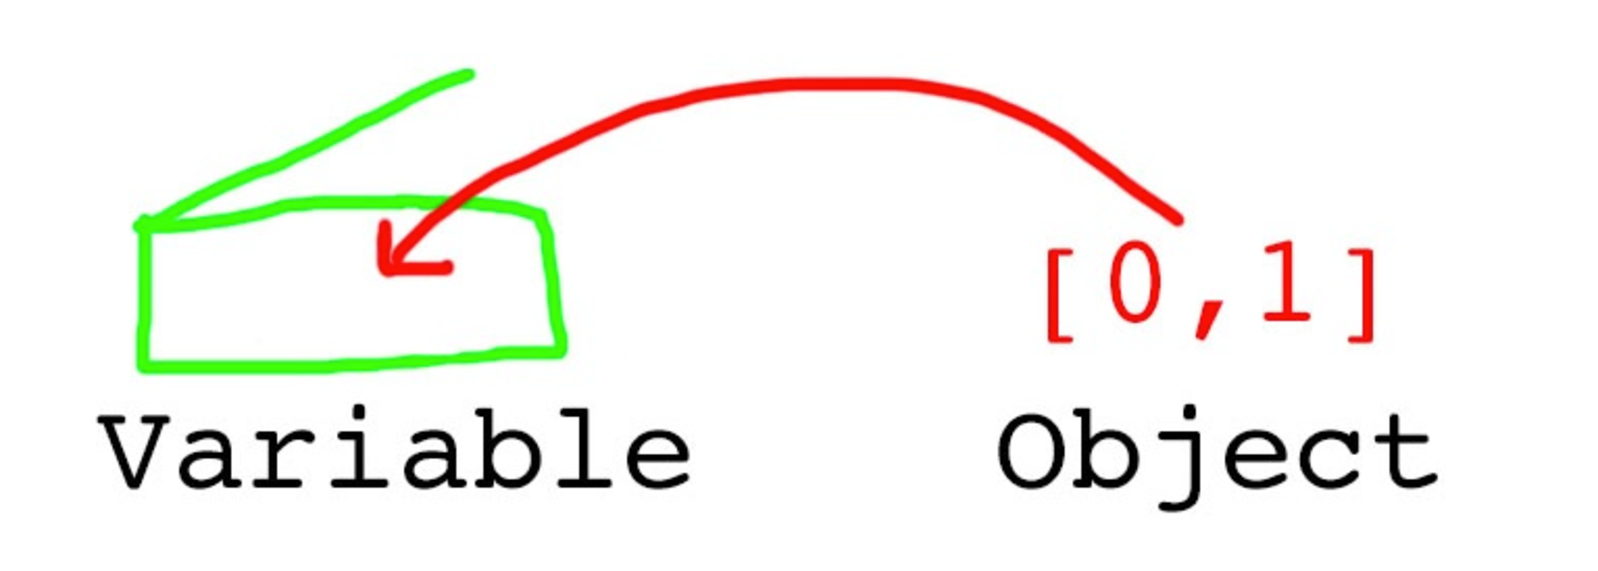
\includegraphics[scale=0.25]{figs/var-objeto-Python.pdf}
 
\tiny{\href{http://robertheaton.com/2014/02/09/pythons-pass-by-object-reference-as-explained-by-philip-k-dick/}{Source}}
\end{center}
\end{frame}

\begin{frame}{Functions}{Global and local variables (VII)}
\textbf{Parameter passing in Phyton}
\medskip
   \begin{columns}
 	   \column{.50\textwidth}
			\centering 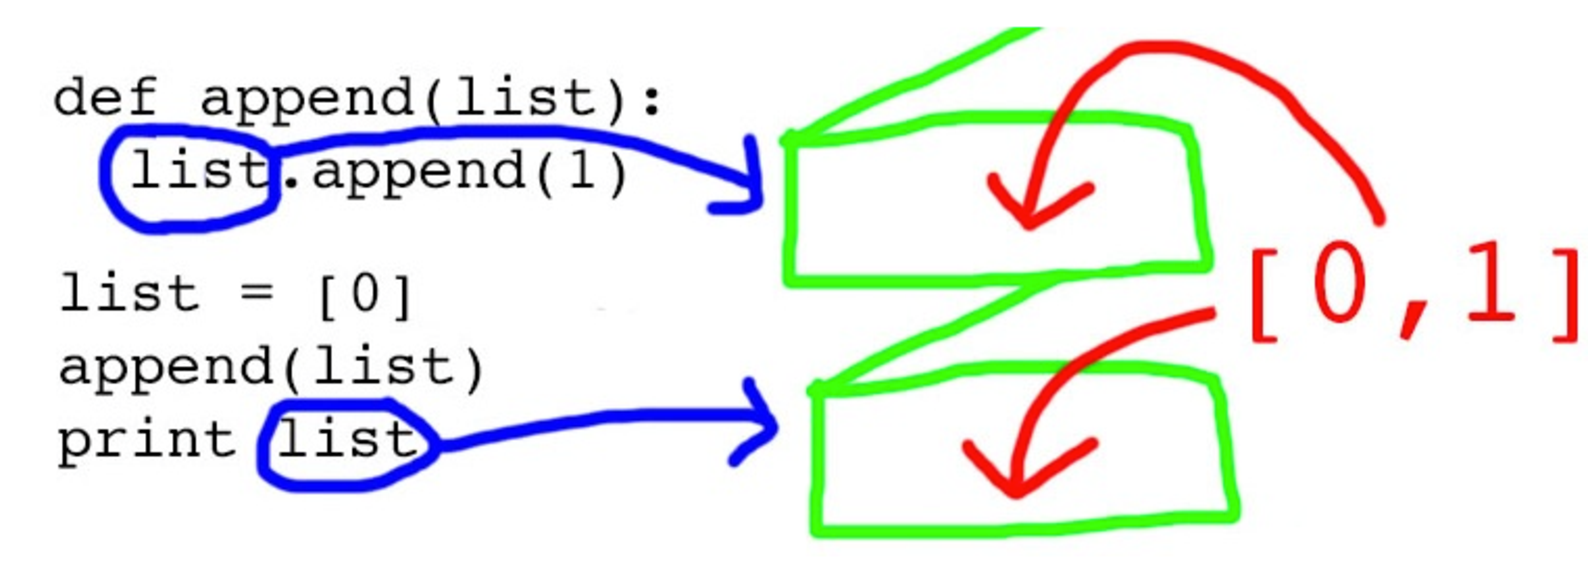
\includegraphics[width=\linewidth]{figs/pasoporreferenciaobjeto1.pdf}
 	   \column{.50\textwidth}
		\centering 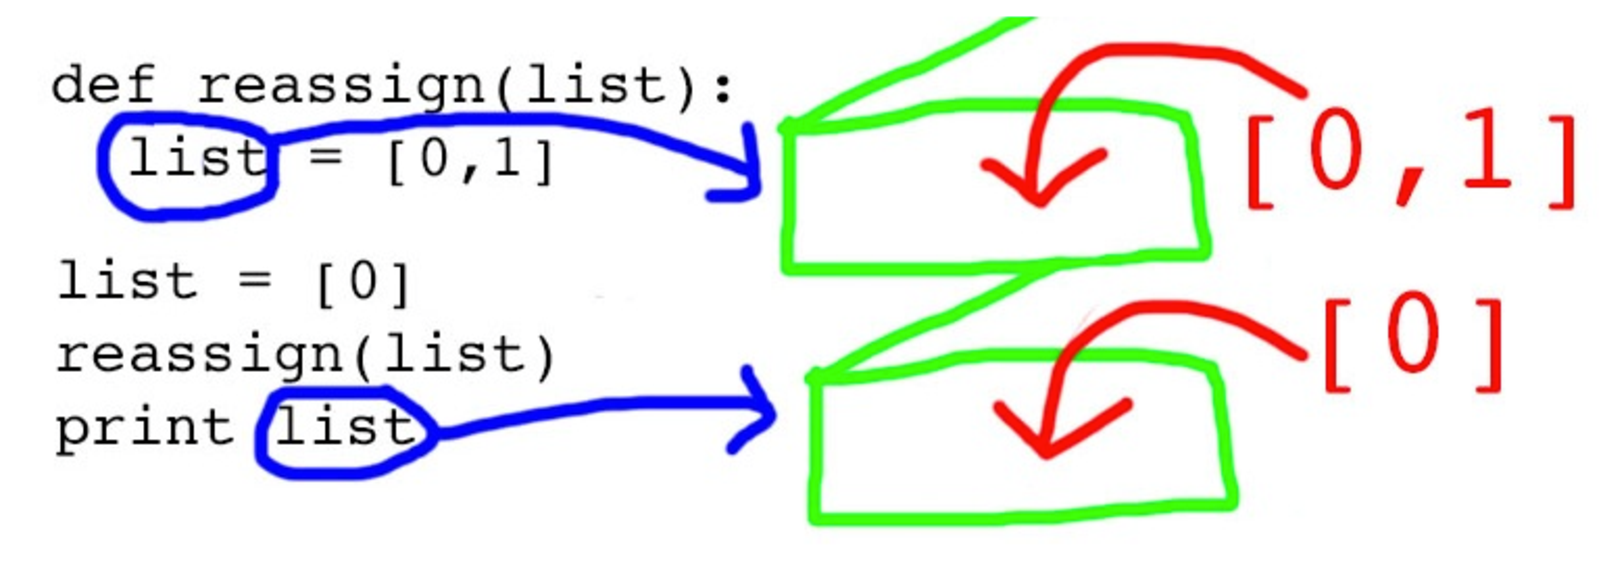
\includegraphics[width=\linewidth]{figs/pasoporreferenciaobjeto2.pdf}
	\end{columns}
	\alert{\href{http://robertheaton.com/2014/02/09/pythons-pass-by-object-reference-as-explained-by-philip-k-dick/}{Want to know more? Click here!}}
\medskip
\begin{block}{Pass-by-object-reference}
\emph{\textit{Object references are passed by value}}
\end{block}
\end{frame}

%\begin{frame}{Functions}{Global and local variables (VIII)}
%Summary:
%\begin{itemize}
%\item \textbf{Global objects}: Objects defined outside the function.
%\item \textbf{Local objects}: Objects defined within the function.
%\item \alert{Global objects} can always be read within a function.
%\item Modification of a global object, \texttt{object}, within a function:
%\begin{itemize}
%\item If \texttt{object} \alert{is immutable} $\rightarrow$ Use \texttt{global object} within the function.
%\item If \texttt{object} \alert{is mutable} $\rightarrow$
%\begin{itemize}
%\item If you want to change by an assignment $\rightarrow$ Use \texttt{global object} within the function.
%\item If you want to chanbe \textbf{using methods} $\rightarrow$ It is not necessary to use \texttt{global object} within the function.
%\end{itemize}
%\end{itemize}
%\end{itemize}
%\end{frame}

\subsection{Default argument values}
\begin{frame}{Functions}{Default argument values (I)}
	Python supports default arguments:
		\begin{itemize}
		\item Poweful and simple feature.
		\item Simpler (and more flexible) function calls.
		\end{itemize}
		\vspace{-0.2cm}
    \begin{columns}
    \column{\textwidth}
		\begin{block}{}
		\vspace{-0.2cm}
		\lstinputlisting{code/default.py}
		\vspace{-0.2cm}
		\end{block}
	\end{columns}
\end{frame}

\begin{frame}{Functions}{Default argument values (II)}
	New Python features
		\begin{itemize}
		\item The \texttt{in} keyword
		\item Exceptions (error handling)
		\end{itemize}

	The function can be invoked in several ways:
		\begin{itemize}
		\item \texttt{ask\_ok('Do you really want to quit')}
		\item \texttt{ask\_ok('OK to overwrite the file?', 2)}
		\item \texttt{ask\_ok('OK to overwrite the file?', 2, 'Come on, yes or no!')}
		\end{itemize}
\end{frame}

\subsection{Keyword arguments}
\begin{frame}{Functions}{Keyword arguments}
	Function arguments can be named:
		\begin{itemize}
		\item It overrides classic positional arguments.
		\item Order does not matter.
		\item Positional arguments must be first.
		\end{itemize}
		\vspace{-0.2cm}
    \begin{columns}
    \column{0.4\textwidth}
		\begin{block}{}
		\vspace{-0.2cm}
		\lstinputlisting{code/keyword.py}
		\vspace{-0.2cm}
		\end{block}

	\column{0.6\textwidth}
		\begin{block}{}
		\vspace{-0.2cm}
		\lstinputlisting{code/keyword-2.py}
		\vspace{-0.2cm}
		\end{block}
	\end{columns}
	\bigskip
	Arbitrary number of arguments:
		\begin{itemize}
			\item Arguments as \texttt{*arg1} and \texttt{**arg2}
			\item Do not worry about it ... right now.
		\end{itemize}
\end{frame}

\section{Coding conventions}
\subsection{Documentation strings}
\begin{frame}{Coding conventions}{Documentation strings (I)}
\vspace{-0.3cm}
	Documentation is important:
		\begin{itemize}
		\item \small {Q: Will you remember why did you wrote that crazy code line?}
		\item \small {A: No, so you must document your code.}
		\item \small {A: Yes, no programmer likes documentating his code.}
		\end{itemize}
	Python provides automatic documentation features:
		\begin{itemize}
		\item \small It can be accessed with \texttt{foo.\_\_doc\_\_} (version 3.X)
		\end{itemize}
   % \begin{columns}
	\vspace{-0.2cm}
  %  \column{\textwidth}
		\scriptsize{
		\begin{exampleblock}{}
		\vspace{-0.4cm}
		\lstinputlisting{code/function-doc.txt}
		\vspace{-0.2cm}
		\end{exampleblock}
		}
%	\end{columns}
\end{frame}

\begin{frame}{Coding conventions}{Documentation strings (II)}
	Documentation conventions:
		\begin{itemize}
		\item The first line should be a summary.
		\item The second line should be blank.
		\item One or more lines with detailed description (arguments, side effects, etc).
		\item Respect indentation.
		\end{itemize}

		\vspace{-0.4cm}
    	\begin{columns}
    	\column{0.7\textwidth}
		\begin{block}{}
		\vspace{-0.2cm}
		\lstinputlisting{code/function-multidoc.py}
		\vspace{-0.2cm}
		\end{block}
		\end{columns}
\end{frame}

\subsection{Coding style}
\begin{frame}{Coding conventions}{Coding style (I)}
	Make your code easy to read using good coding style.\\
	Python coding style convention:
	\begin{itemize}
		\item 4-space indentation, with no tabs.
		\item Maximum 79 characters per code line.
		\item Separate functions and classes with white lines.
		\item Separate large code blocks with white lines.
		\item Use docstrings.
		\item Operators spacing: \texttt{a = f(1, 2) + g(3, 4)}.
		\item Proper use of capitals: 
			\begin{itemize}
			\item Classes: \texttt{CamelCase}
			\item Methods and functions: \texttt{lower\_case\_with\_underscores()}
			\end{itemize}
	\end{itemize}
	\alert{\href{http://mundogeek.net/traducciones/guia-estilo-python.htm}{Want to know more? Click here!}}
\end{frame}

\section{Examples}

\subsection{Example 1}
\begin{frame}[plain,shrink]{Examples}{Example 1: Matrices addition}
	\begin{block}{}
	\vspace{-0.2cm}
	\lstinputlisting{code/matrices.py}
	\vspace{-0.2cm}
	\end{block}
	\vspace{-0.2cm}
	\tiny{\href{http://www.programiz.com/python-programming/examples/add-matrix}{Source}}
\end{frame}

\subsection{Example 2}
\begin{frame}[plain,shrink]{Examples}{Example 2: Calculator}
	\begin{block}{}
	\vspace{-0.2cm}
	\lstinputlisting{code/calculator.py}
	\vspace{-0.2cm}
	\end{block}
	\vspace{-0.2cm}
	\tiny{\href{http://www.programiz.com/python-programming/examples/calculator}{Source}}
\end{frame}

%\subsection{Example 3}
%\begin{frame}[plain,shrink]{Examples}{Example 1: Obtener valores de pixeles}
%Ejemplo de apuntes
%	\begin{block}{}
%	\vspace{-0.2cm}
%	%\lstinputlisting{code/guess.py}
%	\vspace{-0.2cm}
%	\end{block}
%	\vspace{-0.2cm}
%%	\tiny{\href{https://inventwithpython.com/}{Source}}
%\end{frame}

\appendix
\section<Bibliographic references>*{\appendixname}
\subsection<Bibliographic references>*{Bibliographic references}

\begin{frame}[plain,allowframebreaks]
  \frametitle<presentation>{Bibliographic references}

  \begin{thebibliography}{4}

  \beamertemplatebookbibitems
  % libro
   \bibitem{vanRosum}[van Rosum, 2012]
    G. van Rossum, Jr. Fred L. Drake.
    \newblock \emph{Python Tutorial Release 3.2.3, chapter 4}.
    \newblock Python Software Foundation, 2012. 
  % libro
     \bibitem{Bahit}[Bahit, 2008]
     E. Bahit.
    \newblock \emph{Curso: Python para principiantes}.
    \newblock Creative Commons Atribución-NoComercial 3.0, 2012.
    
  % libro
    \bibitem{Swaroop}[Swaroop, 2008]
     C H.  Swaroop.
    \newblock \emph{A Byte of Python}.
    \newblock Creative Commons Attribution-ShareAlike 3.0, 2008.

  \bibitem{Pilgrim}[Pilgrim, 2004]
  M. Pilgrim.
    \newblock \emph{Dive into Python}.
    \newblock Ed. Prentice Hall, 2004.
   
    
 
  \end{thebibliography}
\end{frame}




\end{document}
